\documentclass[conference]{IEEEtran}
\usepackage[T1]{fontenc}
\usepackage{amsmath,amssymb,graphicx,booktabs,cite,url}
\usepackage[hidelinks]{hyperref}
\usepackage{placeins}
\usepackage{stfloats}

% Let LaTeX put more floats on a text page (so they stay near the text that
% cites them) instead of deferring them past the references.
\renewcommand{\topfraction}{0.9}
\renewcommand{\bottomfraction}{0.8}
\renewcommand{\textfraction}{0.07}
\renewcommand{\floatpagefraction}{0.75}
\renewcommand{\dbltopfraction}{0.9}
\renewcommand{\dblfloatpagefraction}{0.75}
\setcounter{topnumber}{3}
\setcounter{bottomnumber}{2}
\setcounter{totalnumber}{5}
\setcounter{dbltopnumber}{3}

% Don't stretch a short column (notably the last one and the bibliography) to
% the full page height; let it end where its content ends.
\raggedbottom

\begin{document}

\title{Do Edits That Fool One Face Recognition Model Fool Others? Measuring the Transfer of PGD Perturbations on LFW}

\author{\IEEEauthorblockN{Dylan Davies (2672598), Sudhir Adjodhya (2652330) and Michael Badenhorst (2652150)}
\IEEEauthorblockA{COMS4036A Computer Vision}}

\maketitle

\begin{abstract}
Photo-cloaking tools protect people from face recognition by adding small, nearly invisible changes, called perturbations, to photos before they are posted. Perturbations generated for a specific face 
recognition model are only useful if they transfer to unseen models. This transfer is evaluated on the 3,000 same-person pairs of the Labeled Faces in the Wild (LFW) benchmark. An InceptionResnetV1
surrogate model was trained from scratch on CASIA-WebFace and used to edit one photo in each pair with Projected Gradient Descent (PGD), an attack that repeatedly adjusts pixels to push the photo's face embedding away from its
original, where no pixel is changed by more than a fraction $\varepsilon$ of the brightness range (0 to 255). Transferability was evaluated across four target models: two pretrained InceptionResnetV1 networks, an 
ArcFace ResNet-50, and a Local Binary Pattern Histogram (LBPH) matcher. For each model, same-person pairs that no longer matched after the perturbation were counted. LBPH, which already fails to match 47.2\% of same-person pairs without any edit, serves as a baseline only. At $\varepsilon = 4/255$ the edit is barely visible: its Structural Similarity Index Measure
(SSIM) is 0.955, where 1.0 means identical. It fools the surrogate on 99.9\% of pairs, but the other deep models are largely unaffected, with none failing to match more than 6.3\% of pairs. Repeating the attack with each pretrained network as the attacker shows that our surrogate 
is the weakest source of transferable edits: at $\varepsilon = 8/255$, edits built against the VGGFace2 model break 82.2\% of the CASIA model's pairs, whereas edits built against our surrogate break 20.6\%. Edits move between the two 
pretrained InceptionResnetV1 networks despite their different training data, while ArcFace resists every attacker (at most 18.8\% of pairs, at a clearly visible $\varepsilon = 16/255$). Random noise, JPEG compression and blur barely affect the deep models, and across three random seeds of the surrogate sweep, no result has a standard deviation above 0.75 percentage points. These results indicate that edits built against one
model give little protection against models with a different architecture, and that transfer is more consistent with shared architecture than with shared training data.
\end{abstract}

\begin{IEEEkeywords}
adversarial examples, transferability, face recognition, privacy, projected gradient descent
\end{IEEEkeywords}

\section{Introduction}
A face recognition model converts a photo of a face into an embedding and judges two photos to show the same person when the embeddings are close. Once photos are posted online, such a 
model can match them without the consent of the person in the picture. Fawkes~\cite{fawkes} and LowKey~\cite{lowkey} offer a means of counteracting this. Both add a 
perturbation to a photo before posting: small changes to pixel values, hard for the human eye to detect, are chosen so that a recogniser misjudges the face. Fawkes poisons the data that a recogniser
trains on, so that a model trained on perturbed photos fails to recognise unperturbed photos of the same person (data poisoning). LowKey applies an adversarial filter so that photos evade commercial face 
recognition systems, including the face detection stage.

A photo that is edited once should resist recognition by every recogniser that later processes the photo. This depends on the transferability of the edit: the extent to which an edit built against one model 
also degrades or fools other models. The extent of this transferability between models is explored in this paper. Although a recogniser trained after the photos are posted can learn to ignore the
perturbation~\cite{radiya}, the work in this report concerns recognisers that are already trained, and transfer is therefore measured on pretrained recognisers.

The edits are generated with Projected Gradient Descent (PGD)~\cite{madry}. A neural network is differentiable, so the gradient of the distance between a 
photo's embedding and the original embedding, taken with respect to the pixels, shows which way to change each pixel to push the embedding further away from the original. PGD takes many small steps in that direction, and after 
each step the result is clipped so that no pixel differs from the original by more than $\varepsilon$. Here $\varepsilon$ is the largest change permitted to any one pixel, expressed as a fraction of the 
full 0 to 255 brightness range, so $\varepsilon = 4/255$ allows each pixel to move by at most 4 brightness levels, which is barely visible. Because the gradient is taken from one model
only, the edit may exploit weaknesses specific to that model and fail on any other.

Two questions govern this investigation: (1) if a photo is edited until one model no longer recognises the person in it, do models the editor never had access to also stop recognising that person? 
(2) Where some models resist the perturbation while others do not, is the difference explained by a shared architecture or by the faces used in training?

The questions are investigated through a controlled experiment on Labeled Faces in the Wild
(LFW)~\cite{lfw}, a benchmark of photo pairs labelled as the same person or different people. One photo of each
same-person pair is edited, and the pairs that a model no longer matches are counted. The edits are built against a
surrogate: an InceptionResnetV1 network~\cite{inceptionv4} trained from scratch on CASIA-WebFace~\cite{casia}. Four
test models are scored on these edits, and each differs from the surrogate in a known way. The \emph{casia} model
matches the surrogate in architecture, loss and training dataset but was trained separately, with a different crop and
training procedure. The \emph{vggface2} model shares the architecture and loss but was trained on different faces
(VGGFace2~\cite{vggface2}). ArcFace~\cite{arcface}, a ResNet-50 trained with an angular margin loss, differs in
architecture, loss and training data. A hand-crafted matcher based on Local Binary Pattern Histograms
(LBPH)~\cite{lbph} adds a baseline that uses no deep learning. In a second experiment, each pretrained model in turn
replaces the surrogate as the attacker. The visibility of each edit is measured with the Structural Similarity Index
Measure (SSIM)~\cite{ssim}, and PGD is compared with random noise, JPEG
compression and blur. The contributions are:
\begin{itemize}
\item a measurement of how often PGD edits built against a from-scratch surrogate stop four unseen models from
matching same-person pairs, over seven edit budgets, with random-noise, JPEG and blur baselines;
\item a comparison in which each of the four neural networks in turn builds the edits and the others are tested on
them, showing that sharing an architecture matters more for transfer than sharing training data;
\item a pipeline in which the same edited photo is cropped separately for each model, with the clean accuracy of
every model checked against its published figure before any attack.
\end{itemize}

\section{Related Work}
Small, targeted input changes can flip the output of a deep network~\cite{szegedy2014}, and gradient-sign
methods~\cite{fgsm} find them in a single step, but PGD~\cite{madry} finds them more reliably by iterating. Such perturbations often transfer between models
trained for the same task~\cite{papernot}, which makes black-box attacks practical. Liu \emph{et
al.}~\cite{liu2017} found that targeted perturbations rarely transfer from one model to another, and that
optimising against an ensemble of models makes them transfer much more often.

Face recognition models map an aligned face crop to an embedding and compare embeddings by distance.
FaceNet~\cite{facenet} trained such embeddings with a triplet loss; ArcFace~\cite{arcface} adds an angular margin to
a softmax loss. Widely used pretrained models include InceptionResnetV1~\cite{inceptionv4} networks trained on
VGGFace2~\cite{vggface2} and CASIA-WebFace~\cite{casia}, distributed with facenet-pytorch~\cite{facenetpytorch},
and InsightFace's~\cite{insightface} ArcFace ResNet-50 trained on WebFace600K, a subset of the WebFace260M
corpus~\cite{webface260m}. LFW remains
the standard verification benchmark, although it is too small to train on~\cite{deepid2} and its subjects are
mostly male and White~\cite{hanjain}.

Fawkes and LowKey use adversarial perturbations as a privacy defence, and both depend on transfer from the model
they optimise against to the one a third party runs. Radiya-Dixit \emph{et al.} show that recognisers trained
later can learn to ignore such perturbations~\cite{radiya}. We isolate the inference-time question and vary architecture and
training data separately.

\section{Method}
\subsection{Threat model}
A user edits one photo of themselves before posting it. They do not know which other photo it will later be
compared with, so the attack pushes the edited photo away from the embedding of its own original. The edit
succeeds against a recogniser if that recogniser no longer matches the edited photo with a different, unedited
photo of the same person.

\subsection{Models}
Table~\ref{tab:models} lists the five models. The surrogate is an InceptionResnetV1 that we trained from scratch
with a softmax cross-entropy loss on CASIA-WebFace, the same architecture and objective as the two facenet-pytorch
models. The \emph{casia} model therefore differs from it only in initialisation, \emph{vggface2} in training data,
and \emph{arcface} in architecture, objective and data. Our LBPH baseline uses local binary pattern
histograms~\cite{lbph}: we divide the crop into an $8\times8$ grid, build a uniform-pattern histogram per cell,
and compare the concatenated histograms with the chi-square distance.

\begin{table}[tb]
\centering
\caption{Models. ``5-pt'' is five-landmark alignment; ``box'' is an MTCNN box crop with a 32-pixel margin.}
\label{tab:models}
\scriptsize
\setlength{\tabcolsep}{3pt}
\begin{tabular}{lllll}
\toprule
Model & Architecture & Training data & Loss & Input \\
\midrule
surrogate & InceptionResnetV1 & CASIA-WebFace (ours) & softmax & 5-pt, 160$^2$ \\
casia & InceptionResnetV1 & CASIA-WebFace & softmax & box, 160$^2$ \\
vggface2 & InceptionResnetV1 & VGGFace2 & softmax & box, 160$^2$ \\
arcface & ResNet-50 & WebFace600K & ArcFace & 5-pt, 112$^2$ \\
lbph & LBP histograms & none & none & 5-pt, 112$^2$ \\
\bottomrule
\end{tabular}
\end{table}

\subsection{Preprocessing}
Each model expects faces cropped and aligned its own way. A wrong crop raises no error; it only lowers accuracy,
which is easy to miss. We run MTCNN~\cite{mtcnn} once on every LFW photo (it found a face in all 7,701) and express each model's crop
as a $2\times3$ affine map from the $250\times250$ photo to the model input: a box crop at $160\times160$ for the
facenet models, the standard InsightFace~\cite{insightface} five-point alignment at $112\times112$ for ArcFace and LBPH, and a
five-point alignment at $160\times160$ for the surrogate, using the landmark positions MTCNN finds on its CASIA
training crops. The crops are applied with a differentiable bilinear warp, so the surrogate's own cropping sits
inside the attack. Every edit is made on the full photo, and every model crops the same edited photo.

\subsection{Verification protocol}
A pair is accepted as the same person when the distance between embeddings (cosine for the deep models,
chi-square for LBPH) is below a threshold. Following the LFW protocol~\cite{lfw}, each model's threshold for a fold is fitted
on the clean pairs of the other nine folds. We keep these clean thresholds fixed when scoring edited photos, so
$\varepsilon = 0$ gives each model's ordinary error rate.

\subsection{Attack}
For a photo $x$ with surrogate embedding $f(x)$, PGD~\cite{madry} starts from $x$ plus uniform noise in
$[-\varepsilon, \varepsilon]$ and repeats
\begin{equation}
x^{t+1} = \Pi_{\varepsilon}\!\left(x^{t} + \alpha \,\mathrm{sign}\, \nabla_{x}\, d\big(f(x^{t}), f(x)\big)\right),
\end{equation}
where $d$ is the cosine distance and $\Pi_\varepsilon$ projects onto the $L_\infty$ ball of radius $\varepsilon$
around $x$ and onto valid pixel values. We use 20 steps with $\alpha = 2.5\varepsilon/20$, and round the result to
8 bits before scoring, as a posted photo would be. We sweep $\varepsilon \in \{0, 0.5, 1, 2, 4, 8, 16\}/255$.

\subsection{Baselines and metrics}
Random sign noise of size $\varepsilon$ on every pixel tests whether the optimisation matters. Saving the edited
photo as JPEG at quality 75 tests whether ordinary recompression removes the edit. JPEG compression (quality 90 to
30) and Gaussian blur ($\sigma$ = 0.5 to 3 pixels) of the clean photo are edits any user could make for free.

Our measure is the \emph{unmatched share}: the fraction of the 3,000 same-person pairs that a model no longer
accepts after photo $a$ of each pair is edited, averaged over the ten folds. SSIM~\cite{ssim} between the edited
and original photo measures how visible the edit is.

\section{Experimental Setup}
LFW View~2 holds 6,000 fixed pairs in ten folds. We use the published pairs unchanged, with no corrections of
our own. The surrogate was trained for 30 epochs on CASIA-WebFace~\cite{casia} (465,498 aligned images
of 10,072 identities in our copy, after holding out 500 identities for validation) with SGD (Nesterov momentum 0.9, weight decay $5\times10^{-4}$), a one-cycle
schedule~\cite{onecycle} peaking at a
learning rate of 0.1, batch size 256, bf16 mixed precision and random horizontal flips. Training took about
1.5~hours on one RTX~5070~Ti. We kept the epoch (27) with the best verification accuracy on the held-out
identities (90.9\%), never on LFW. It reached 98.28\% clean LFW accuracy, against the 99.05\% facenet-pytorch reports~\cite{facenetpytorch} for the pretrained \emph{casia} model
trained on the same data.

Because a misaligned crop lowers accuracy without any error, we checked every model against its published LFW
accuracy before attacking (Table~\ref{tab:valid}). We chose the facenet crop margin from $\{0, 14, 32, 44\}$
pixels by clean accuracy; 32 was best for both models. The three pretrained deep models land within 0.32
points of their published figures. For the cross-attacker experiments we converted ArcFace from ONNX to PyTorch
with onnx2torch so that gradients flow through it; the converted model reproduces the original's accuracy.

\begin{table}[tb]
\centering
\caption{Clean LFW View 2 accuracy (mean $\pm$ std over 10 folds) against the figures published for the same
checkpoints: facenet-pytorch's model table~\cite{facenetpytorch} for \emph{casia} and \emph{vggface2},
InsightFace's model zoo~\cite{insightface} for the \emph{buffalo\_l} ArcFace model.}
\label{tab:valid}
\footnotesize
\begin{tabular}{lrrr}
\toprule
Model & Ours & Published & Gap (pts) \\
\midrule
surrogate & 98.28\% $\pm$ 0.61\% & -- & -- \\
casia & 98.73\% $\pm$ 0.64\% & 99.05\% & -0.32 \\
vggface2 & 99.37\% $\pm$ 0.33\% & 99.65\% & -0.28 \\
arcface & 99.85\% $\pm$ 0.17\% & 99.83\% & +0.02 \\
lbph & 67.03\% $\pm$ 1.03\% & -- & -- \\
\bottomrule
\end{tabular}
\end{table}

\section{Results}
\subsection{Transfer from the surrogate}
Table~\ref{tab:main} and Fig.~\ref{fig:main} give the main result. The surrogate stops matching quickly: from
2.0\% of pairs with no edit to 75.1\% at $\varepsilon = 2/255$, where the edit is essentially invisible (SSIM
0.986), and 99.9\% from $4/255$ up. The other deep models hardly move at these budgets. At $4/255$ \emph{casia}
goes from 1.8\% to 6.3\%, \emph{vggface2} from 0.8\% to 1.7\% and ArcFace from 0.3\% to 0.4\%. Substantial
transfer appears only at $16/255$, where SSIM has fallen to 0.659 and the edit is plain to see. There
\emph{casia} loses 60.7\% of pairs, \emph{vggface2} 14.6\% and ArcFace 1.0\%.

With our surrogate as the attacker, shared training data looks decisive: \emph{casia}, trained on the same faces,
loses 4.2 times as many pairs at $16/255$ as \emph{vggface2}. Section~\ref{sec:cross} shows that this reading
does not survive a change of attacker.

\begin{table*}[tb]
\centering
\caption{Unmatched share of same-person pairs (mean $\pm$ std over folds) after PGD against the surrogate.
$\varepsilon = 0$ is each model's baseline error. SSIM is between edited and original photo.}
\label{tab:main}
\footnotesize
\begin{tabular}{lrrrrrr}
\toprule
$\varepsilon$ & surrogate & casia & vggface2 & arcface & lbph & SSIM \\
\midrule
0/255 & 2.0\% $\pm$ 1.2\% & 1.8\% $\pm$ 1.4\% & 0.8\% $\pm$ 0.7\% & 0.3\% $\pm$ 0.4\% & 47.2\% $\pm$ 2.1\% & 1.000 \\
0.5/255 & 5.1\% $\pm$ 1.8\% & 1.9\% $\pm$ 1.4\% & 0.9\% $\pm$ 0.7\% & 0.3\% $\pm$ 0.4\% & 45.1\% $\pm$ 1.7\% & 0.999 \\
1/255 & 14.6\% $\pm$ 2.5\% & 2.1\% $\pm$ 1.2\% & 0.9\% $\pm$ 0.9\% & 0.3\% $\pm$ 0.4\% & 42.9\% $\pm$ 2.0\% & 0.996 \\
2/255 & 75.1\% $\pm$ 3.1\% & 2.6\% $\pm$ 1.4\% & 1.0\% $\pm$ 0.9\% & 0.3\% $\pm$ 0.5\% & 40.4\% $\pm$ 2.2\% & 0.986 \\
4/255 & 99.9\% $\pm$ 0.1\% & 6.3\% $\pm$ 2.0\% & 1.7\% $\pm$ 1.0\% & 0.4\% $\pm$ 0.5\% & 39.0\% $\pm$ 1.9\% & 0.955 \\
8/255 & 100.0\% $\pm$ 0.0\% & 20.6\% $\pm$ 2.9\% & 3.5\% $\pm$ 1.6\% & 0.5\% $\pm$ 0.5\% & 44.9\% $\pm$ 2.3\% & 0.860 \\
16/255 & 100.0\% $\pm$ 0.0\% & 60.7\% $\pm$ 4.0\% & 14.6\% $\pm$ 2.3\% & 1.0\% $\pm$ 0.7\% & 65.6\% $\pm$ 2.0\% & 0.659 \\
\bottomrule
\end{tabular}
\end{table*}

\begin{figure}[tb]
\centering
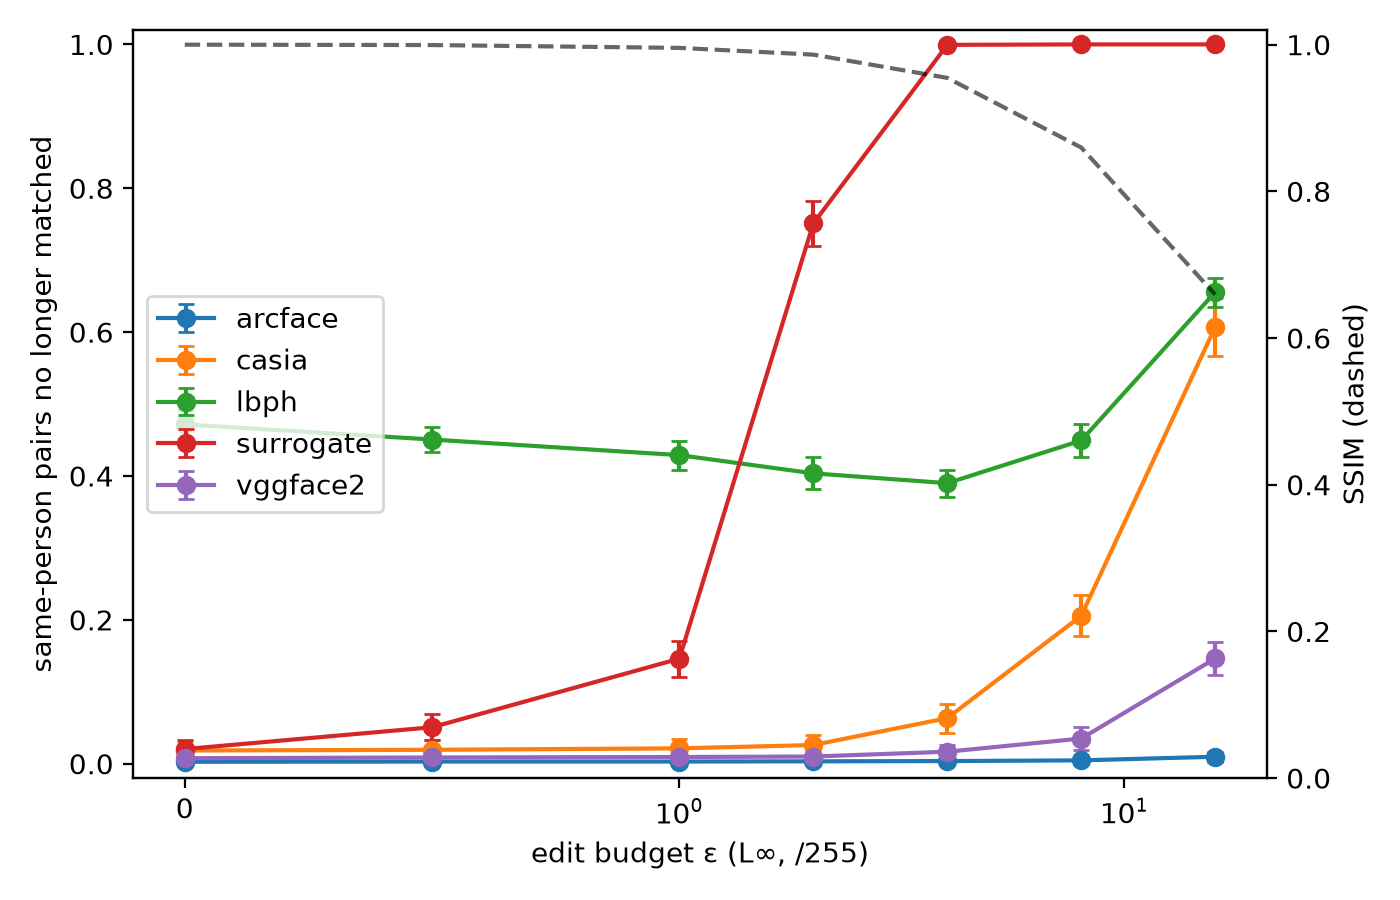
\includegraphics[width=\columnwidth]{figures/main_result.png}
\caption{Unmatched share against edit budget for PGD against the surrogate, one line per model (error bars: std
over folds). Dashed: SSIM (right axis).}
\label{fig:main}
\end{figure}

\subsection{Baselines}
Random noise does little even though it is more visible than PGD at the same budget (Table~\ref{tab:base},
Fig.~\ref{fig:compare}). At $\varepsilon = 16/255$, noise (SSIM 0.462) makes the surrogate fail to match
only 6.6\% of pairs, against 100.0\% for PGD (SSIM 0.659), and \emph{casia} only 4.3\%, against 60.7\%. JPEG at quality 75 after editing weakens small edits, cutting the surrogate's unmatched
share at $2/255$ from 75.1\% to 32.3\%, but edits of $4/255$ and above survive it (96.0\% at $4/255$). Free edits
barely register: JPEG at quality 30 leaves the surrogate at 2.1\%, and only strong blur ($\sigma = 3$ pixels, SSIM
0.790) has an effect, 21.3\% for the surrogate and 16.6\% for \emph{casia}.

\begin{table}[tb]
\centering
\caption{Unmatched share under baseline edits (S surrogate, C casia, V vggface2, A arcface, L lbph).}
\label{tab:base}
\scriptsize
\setlength{\tabcolsep}{2.5pt}
\begin{tabular}{llrrrrrr}
\toprule
Edit & Strength & S & C & V & A & L & SSIM \\
\midrule
Noise & $\varepsilon$ = 8/255 & 2.8\% & 2.4\% & 0.9\% & 0.3\% & 65.4\% & 0.713 \\
Noise & $\varepsilon$ = 16/255 & 6.6\% & 4.3\% & 1.4\% & 0.4\% & 90.1\% & 0.462 \\
PGD + JPEG 75 & $\varepsilon$ = 2/255 & 32.3\% & 2.7\% & 1.1\% & 0.3\% & 39.6\% & 0.968 \\
PGD + JPEG 75 & $\varepsilon$ = 4/255 & 96.0\% & 5.5\% & 1.6\% & 0.4\% & 36.6\% & 0.959 \\
PGD + JPEG 75 & $\varepsilon$ = 16/255 & 100.0\% & 51.8\% & 12.6\% & 0.8\% & 48.9\% & 0.819 \\
JPEG & q = 50 & 2.3\% & 1.9\% & 0.8\% & 0.3\% & 49.2\% & 0.952 \\
JPEG & q = 30 & 2.1\% & 2.0\% & 0.8\% & 0.3\% & 54.9\% & 0.927 \\
Blur & $\sigma$ = 2 & 6.1\% & 5.2\% & 2.1\% & 0.3\% & 97.4\% & 0.876 \\
Blur & $\sigma$ = 3 & 21.3\% & 16.6\% & 6.8\% & 0.7\% & 99.6\% & 0.790 \\
\bottomrule
\end{tabular}
\end{table}

\begin{figure*}[tb]
\centering
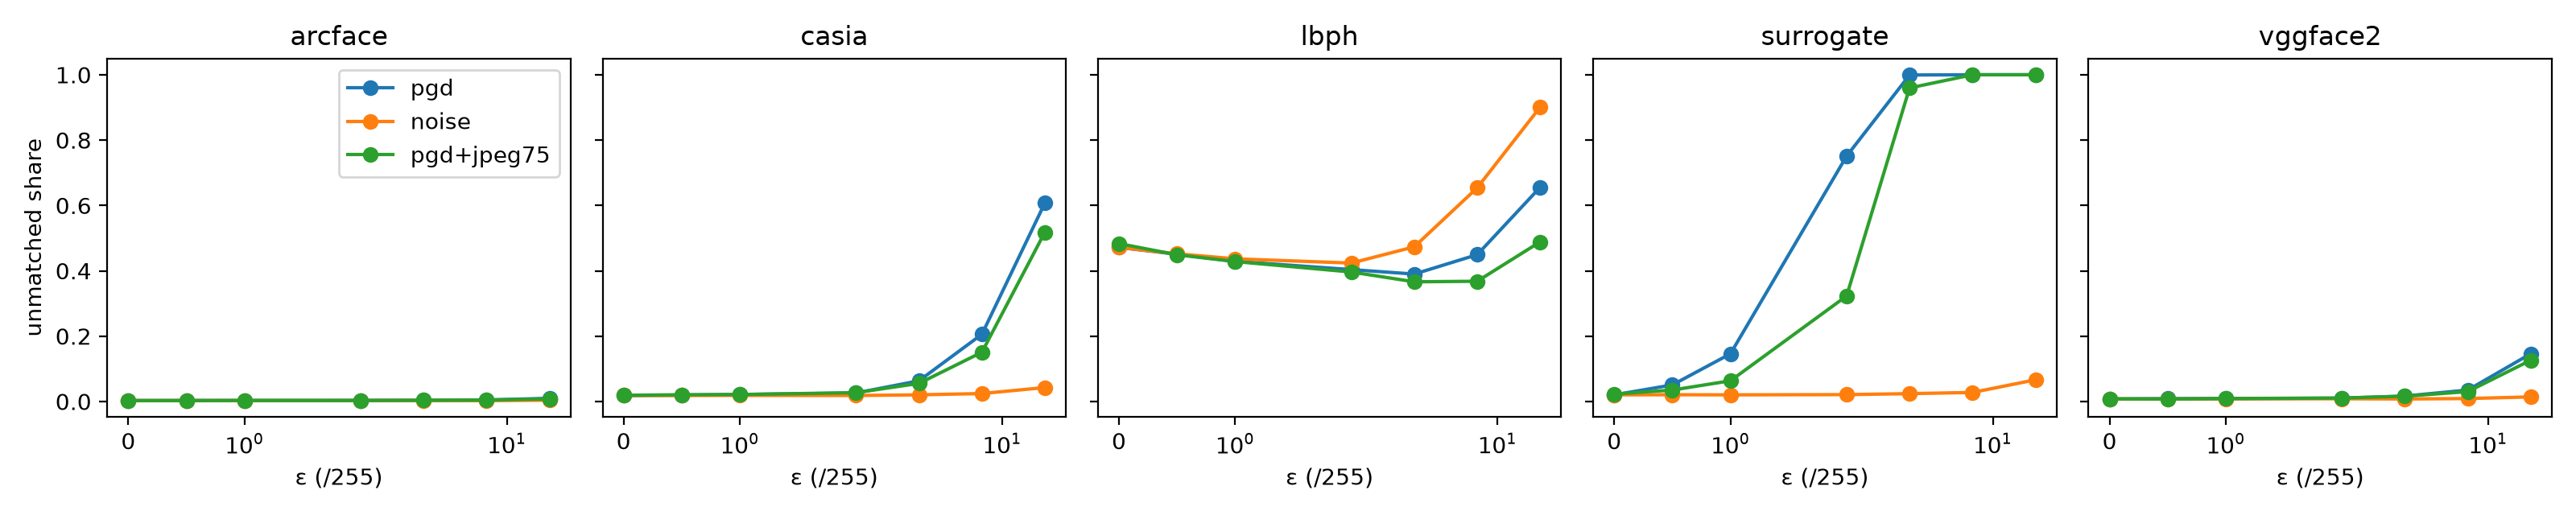
\includegraphics[width=\textwidth]{figures/edit_comparison.png}
\caption{PGD against the surrogate compared with random noise of the same budget and with PGD followed by JPEG at
quality 75, one panel per scored model.}
\label{fig:compare}
\end{figure*}

\subsection{Stability across seeds}
The random seed sets PGD's starting point and the noise baseline. We repeated the full surrogate sweep with two
more seeds. Across the three seeds the standard deviation of every averaged result stayed at or below 0.75
percentage points, far smaller than the differences between models.

\subsection{Every deep model as the attacker}\label{sec:cross}
Low transfer could be a property of our surrogate rather than of transfer in general. To test this we repeated the
attack with \emph{casia}, \emph{vggface2} and ArcFace as the attacker and scored all five models
(Table~\ref{tab:matrix}, Fig.~\ref{fig:matrix}). Edits are equally visible whichever model builds them: at every
budget their SSIM differs by at most 0.004.

Our surrogate is the weakest attacker. At $\varepsilon = 8/255$ its edits break 20.6\% of \emph{casia}'s pairs,
while edits built against \emph{vggface2} break 82.2\%. It is also the easiest model to fool: edits from
\emph{casia} and \emph{vggface2} break 81.2\% and 72.0\% of its pairs at the same budget.

Architecture predicts transfer better than training data. The three InceptionResnetV1 models fool one another
even when trained on different faces: \emph{vggface2}~$\to$~\emph{casia} reaches 82.2\% at $8/255$ and 98.7\% at
$16/255$. ArcFace resists every attacker; the strongest, \emph{vggface2}, reaches 18.8\% and only at $16/255$.
ArcFace's own edits transfer moderately to the others (55.3\% surrogate, 45.9\% \emph{casia}, 21.4\%
\emph{vggface2} at $16/255$).

Transfer is also lopsided. At $8/255$, \emph{vggface2}~$\to$~\emph{casia} (82.2\%) is much stronger than
\emph{casia}~$\to$~\emph{vggface2} (32.0\%). At the nearly invisible $4/255$, the strongest transfer between two
different deep models is \emph{casia}~$\to$~\emph{surrogate} at 27.1\%, and at $2/255$ none exceeds 5.1\%.

\begin{table}[tb]
\centering
\caption{Unmatched share when the edit is built against the attacker (row) and scored on the target (column).
Bold: attacker scored on itself.}
\label{tab:matrix}
\scriptsize
\setlength{\tabcolsep}{2pt}
\begin{tabular}{lrrrrrr}
\toprule
Attacker $\downarrow$ / target $\rightarrow$ & surrogate & casia & vggface2 & arcface & lbph & SSIM \\
\midrule
\multicolumn{7}{l}{\emph{$\varepsilon$ = 4/255}} \\
surrogate & \textbf{99.9\%} & 6.3\% & 1.7\% & 0.4\% & 39.0\% & 0.955 \\
casia & 27.1\% & \textbf{98.9\%} & 6.4\% & 0.4\% & 40.3\% & 0.953 \\
vggface2 & 19.4\% & 22.7\% & \textbf{95.3\%} & 0.5\% & 40.1\% & 0.954 \\
arcface & 7.8\% & 5.5\% & 2.1\% & \textbf{95.9\%} & 41.5\% & 0.953 \\
\multicolumn{7}{l}{\emph{$\varepsilon$ = 8/255}} \\
surrogate & \textbf{100.0\%} & 20.6\% & 3.5\% & 0.5\% & 44.9\% & 0.860 \\
casia & 81.2\% & \textbf{100.0\%} & 32.0\% & 1.3\% & 45.6\% & 0.856 \\
vggface2 & 72.0\% & 82.2\% & \textbf{100.0\%} & 3.7\% & 42.6\% & 0.857 \\
arcface & 24.1\% & 16.3\% & 6.2\% & \textbf{100.0\%} & 46.5\% & 0.856 \\
\multicolumn{7}{l}{\emph{$\varepsilon$ = 16/255}} \\
surrogate & \textbf{100.0\%} & 60.7\% & 14.6\% & 1.0\% & 65.6\% & 0.659 \\
casia & 97.7\% & \textbf{100.0\%} & 75.5\% & 7.3\% & 65.5\% & 0.656 \\
vggface2 & 96.7\% & 98.7\% & \textbf{100.0\%} & 18.8\% & 60.1\% & 0.657 \\
arcface & 55.3\% & 45.9\% & 21.4\% & \textbf{100.0\%} & 65.5\% & 0.655 \\
\bottomrule
\end{tabular}
\end{table}

\begin{figure*}[tb]
\centering
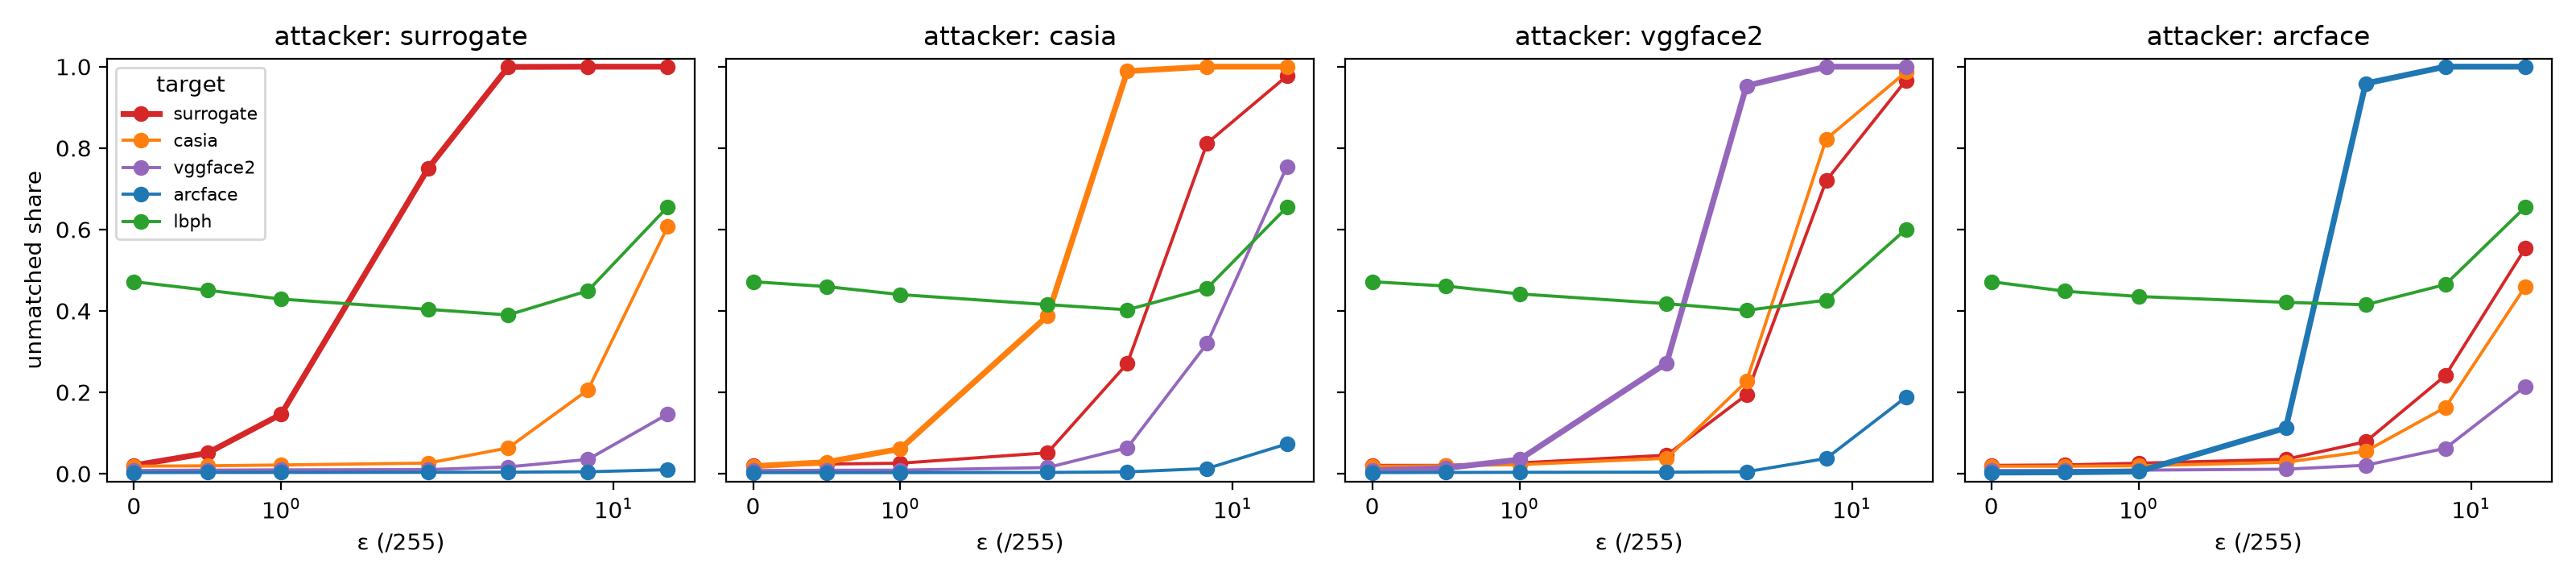
\includegraphics[width=\textwidth]{figures/attacker_transfer.png}
\caption{Unmatched share against $\varepsilon$ for each attacker (one panel each), one line per target. The thick
line is the attacker scored on itself.}
\label{fig:matrix}
\end{figure*}

\subsection{What the edits look like}
Fig.~\ref{fig:example}, at the end of the paper, shows one LFW pair (Vanessa Incontrada) edited by each attacker. At 2--4/255 the edits are hard to
see; at $16/255$ they add a visible grain, mostly on skin. Fig.~\ref{fig:pert} shows the change alone. The
pretrained attackers' edits follow the eyes, brows, mouth and outline of the face, while the surrogate's looks like
texture with little facial structure. Each edit stays inside its attacker's crop; outside it, only PGD's random
start remains.

\section{Discussion}
Our first experiment, with only our surrogate as the attacker, suggested that edits transfer mainly to models that
share training data. The cross-attacker results overturn that reading. Edits transfer readily among the three
InceptionResnetV1 models whatever their training data, and ArcFace, the one model with a different architecture,
is barely touched by any of them. On the proposal's question of architecture against data, the evidence favours
architecture.

We did not test why our surrogate is a weak attacker, but three explanations fit what we saw. It may overfit:
training accuracy reached 97.6\% while LFW accuracy levelled off, even though we kept the epoch that was best on
held-out identities. Its crop geometry differs from the facenet models', which use a box crop; ArcFace, which shares the
landmark-based alignment, transfers better to the surrogate (24.1\%) than to \emph{casia} (16.3\%) at
$8/255$. It also had far less training than the pretrained models.

LBPH requires a more cautious interpretation. Its clean accuracy is only 67.0\%, and its errors fall mostly on same-person pairs: it fails to match 47.2\% of them before any edit.
Random noise at $16/255$ breaks 90.1\% of its pairs against 65.6\% for PGD, and blur at $\sigma = 3$ breaks
99.6\%. It reacts to any change in fine texture, so we treat it as a baseline rather than as evidence of transfer.

This is discouraging for privacy tools. Whether an edit protects someone depends on which model it was built
against, and the protection is much weaker against a model with a different architecture. At a nearly invisible
budget, even the best-matched pair of models transfers to only 27.1\% of pairs.

\section{Limitations}
We used one attack and did not try ensemble attacks~\cite{liu2017}, which usually transfer better. Only the
surrogate attacker was repeated over three seeds. Landmarks are detected on the clean photo and reused for its
edited versions, whereas a deployed system would detect the face again. PGD on the GPU is not bit-for-bit
reproducible even with a fixed seed; re-running the example edits changed 3 of 300 fooled-or-matched decisions,
all for models sitting at their threshold. PGD's random start leaves noise outside the attacker's crop, which
lowers SSIM slightly and equally for every attacker. Finally, we did not check whether protection is equally
effective across demographic groups, which matters given LFW's skew~\cite{hanjain}.

\section{Conclusion}
PGD edits built against a from-scratch face recognition model transfer poorly to models its author never used.
Changing the attacker shows that this is partly a weakness of our surrogate: edits built against a pretrained
InceptionResnetV1 transfer strongly to other networks with that architecture, even across training sets. A
different architecture resists edits from every attacker we tried until the edit is clearly visible. A privacy
edit made once against one model should not be expected to protect against an unknown recogniser.


\FloatBarrier
\begin{thebibliography}{99}
\bibitem{fawkes} S.~Shan, E.~Wenger, J.~Zhang, H.~Li, H.~Zheng, and B.~Y. Zhao, ``Fawkes: Protecting privacy
against unauthorized deep learning models,'' in \emph{Proc. 29th USENIX Security Symp.}, 2020, pp. 1589--1604.
\bibitem{lowkey} V.~Cherepanova, M.~Goldblum, H.~Foley, S.~Duan, J.~Dickerson, G.~Taylor, and T.~Goldstein,
``LowKey: Leveraging adversarial attacks to protect social media users from facial recognition,'' in \emph{Proc.
Int. Conf. Learn. Represent. (ICLR)}, 2021.
\bibitem{radiya} E.~Radiya-Dixit, N.~Carlini, S.~Hong, and F.~Tram\`er, ``Data poisoning won't save you from facial
recognition,'' in \emph{Proc. Int. Conf. Learn. Represent. (ICLR)}, 2022.
\bibitem{szegedy2014} C.~Szegedy, W.~Zaremba, I.~Sutskever, J.~Bruna, D.~Erhan, I.~Goodfellow, and R.~Fergus,
``Intriguing properties of neural networks,'' in \emph{Proc. Int. Conf. Learn. Represent. (ICLR)}, 2014.
\bibitem{fgsm} I.~J. Goodfellow, J.~Shlens, and C.~Szegedy, ``Explaining and harnessing adversarial examples,'' in
\emph{Proc. Int. Conf. Learn. Represent. (ICLR)}, 2015.
\bibitem{madry} A.~Madry, A.~Makelov, L.~Schmidt, D.~Tsipras, and A.~Vladu, ``Towards deep learning models resistant
to adversarial attacks,'' in \emph{Proc. Int. Conf. Learn. Represent. (ICLR)}, 2018.
\bibitem{papernot} N.~Papernot, P.~McDaniel, and I.~Goodfellow, ``Transferability in machine learning: From
phenomena to black-box attacks using adversarial samples,'' arXiv:1605.07277, 2016.
\bibitem{liu2017} Y.~Liu, X.~Chen, C.~Liu, and D.~Song, ``Delving into transferable adversarial examples and
black-box attacks,'' in \emph{Proc. Int. Conf. Learn. Represent. (ICLR)}, 2017.
\bibitem{lfw} G.~B. Huang, M.~Ramesh, T.~Berg, and E.~Learned-Miller, ``Labeled Faces in the Wild: A database for
studying face recognition in unconstrained environments,'' Univ. Massachusetts, Amherst, Tech. Rep. 07-49, 2007.
\bibitem{casia} D.~Yi, Z.~Lei, S.~Liao, and S.~Z. Li, ``Learning face representation from scratch,''
arXiv:1411.7923, 2014.
\bibitem{vggface2} Q.~Cao, L.~Shen, W.~Xie, O.~M. Parkhi, and A.~Zisserman, ``VGGFace2: A dataset for recognising
faces across pose and age,'' in \emph{Proc. IEEE Int. Conf. Autom. Face Gesture Recognit. (FG)}, 2018,
pp. 67--74.
\bibitem{facenet} F.~Schroff, D.~Kalenichenko, and J.~Philbin, ``FaceNet: A unified embedding for face recognition
and clustering,'' in \emph{Proc. IEEE Conf. Comput. Vis. Pattern Recognit. (CVPR)}, 2015, pp. 815--823.
\bibitem{inceptionv4} C.~Szegedy, S.~Ioffe, V.~Vanhoucke, and A.~A. Alemi, ``Inception-v4, Inception-ResNet and the
impact of residual connections on learning,'' in \emph{Proc. AAAI Conf. Artif. Intell.}, 2017, pp. 4278--4284.
\bibitem{arcface} J.~Deng, J.~Guo, N.~Xue, and S.~Zafeiriou, ``ArcFace: Additive angular margin loss for deep face
recognition,'' in \emph{Proc. IEEE/CVF Conf. Comput. Vis. Pattern Recognit. (CVPR)}, 2019, pp. 4690--4699.
\bibitem{webface260m} Z.~Zhu, G.~Huang, J.~Deng, Y.~Ye, J.~Huang, X.~Chen, J.~Zhu, T.~Yang, J.~Lu, D.~Du, and
J.~Zhou, ``WebFace260M: A benchmark unveiling the power of million-scale deep face recognition,'' in \emph{Proc.
IEEE/CVF Conf. Comput. Vis. Pattern Recognit. (CVPR)}, 2021.
\bibitem{lbph} T.~Ahonen, A.~Hadid, and M.~Pietik\"ainen, ``Face description with local binary patterns:
Application to face recognition,'' \emph{IEEE Trans. Pattern Anal. Mach. Intell.}, vol.~28, no.~12,
pp. 2037--2041, 2006.
\bibitem{mtcnn} K.~Zhang, Z.~Zhang, Z.~Li, and Y.~Qiao, ``Joint face detection and alignment using multitask
cascaded convolutional networks,'' \emph{IEEE Signal Process. Lett.}, vol.~23, no.~10, pp. 1499--1503, 2016.
\bibitem{ssim} Z.~Wang, A.~C. Bovik, H.~R. Sheikh, and E.~P. Simoncelli, ``Image quality assessment: From error
visibility to structural similarity,'' \emph{IEEE Trans. Image Process.}, vol.~13, no.~4, pp. 600--612, 2004.
\bibitem{facenetpytorch} T.~Esler, ``facenet-pytorch,'' GitHub repository, 2019. [Online]. Available:
\url{https://github.com/timesler/facenet-pytorch}
\bibitem{deepid2} Y.~Sun, Y.~Chen, X.~Wang, and X.~Tang, ``Deep learning face representation by joint
identification-verification,'' in \emph{Proc. Adv. Neural Inf. Process. Syst. (NeurIPS)}, 2014.
\bibitem{insightface} J.~Guo and J.~Deng, ``InsightFace: 2D and 3D face analysis project,'' GitHub repository,
model zoo. [Online]. Available: \url{https://github.com/deepinsight/insightface}
\bibitem{onecycle} L.~N. Smith and N.~Topin, ``Super-convergence: Very fast training of neural networks using
large learning rates,'' arXiv:1708.07120, 2018.
\bibitem{hanjain} H.~Han and A.~K. Jain, ``Age, gender and race estimation from unconstrained face images,''
Michigan State Univ., Tech. Rep. MSU-CSE-14-5, 2014.
\end{thebibliography}

% The two large example figures go on their own page on their own page at the very end, after the references, so
% neither breaks into the body text.

\begin{figure*}[p]
\centering
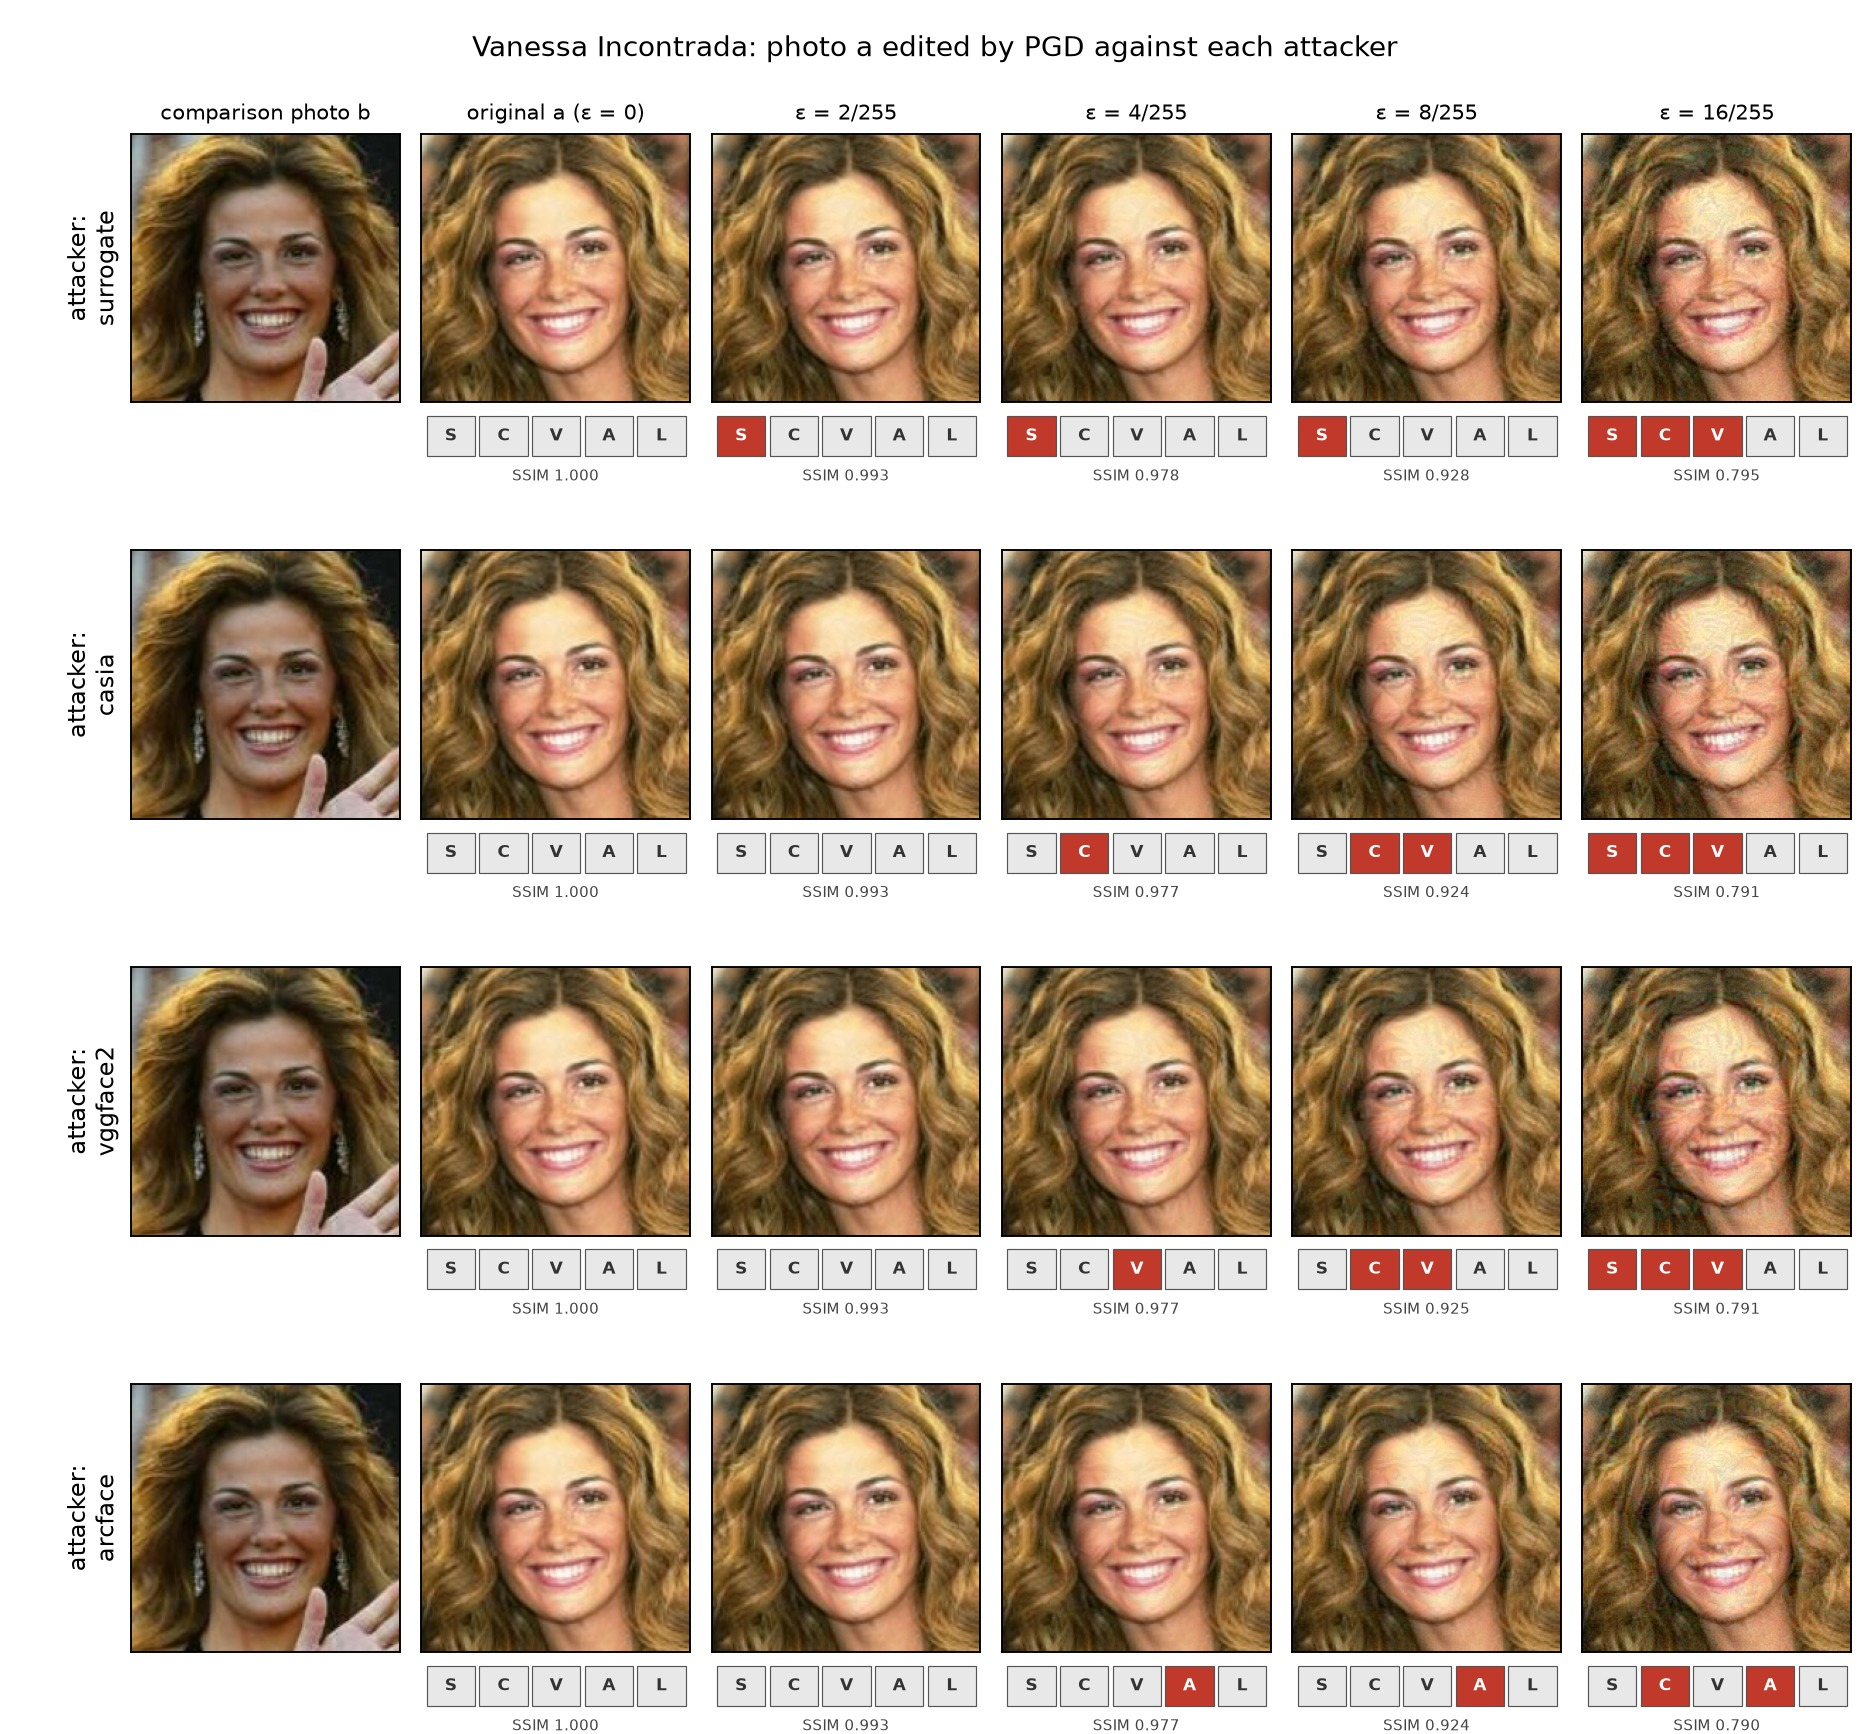
\includegraphics[width=0.80\textwidth]{figures/example_0.jpg}
\caption{Photo $a$ of one pair edited against each attacker (rows) at each budget (columns), with the comparison
photo $b$ on the left. Tags under each photo: models fooled (red) or still matching (grey); S surrogate, C casia,
V vggface2, A arcface, L lbph.}
\label{fig:example}
\end{figure*}

\begin{figure*}[p]
\centering
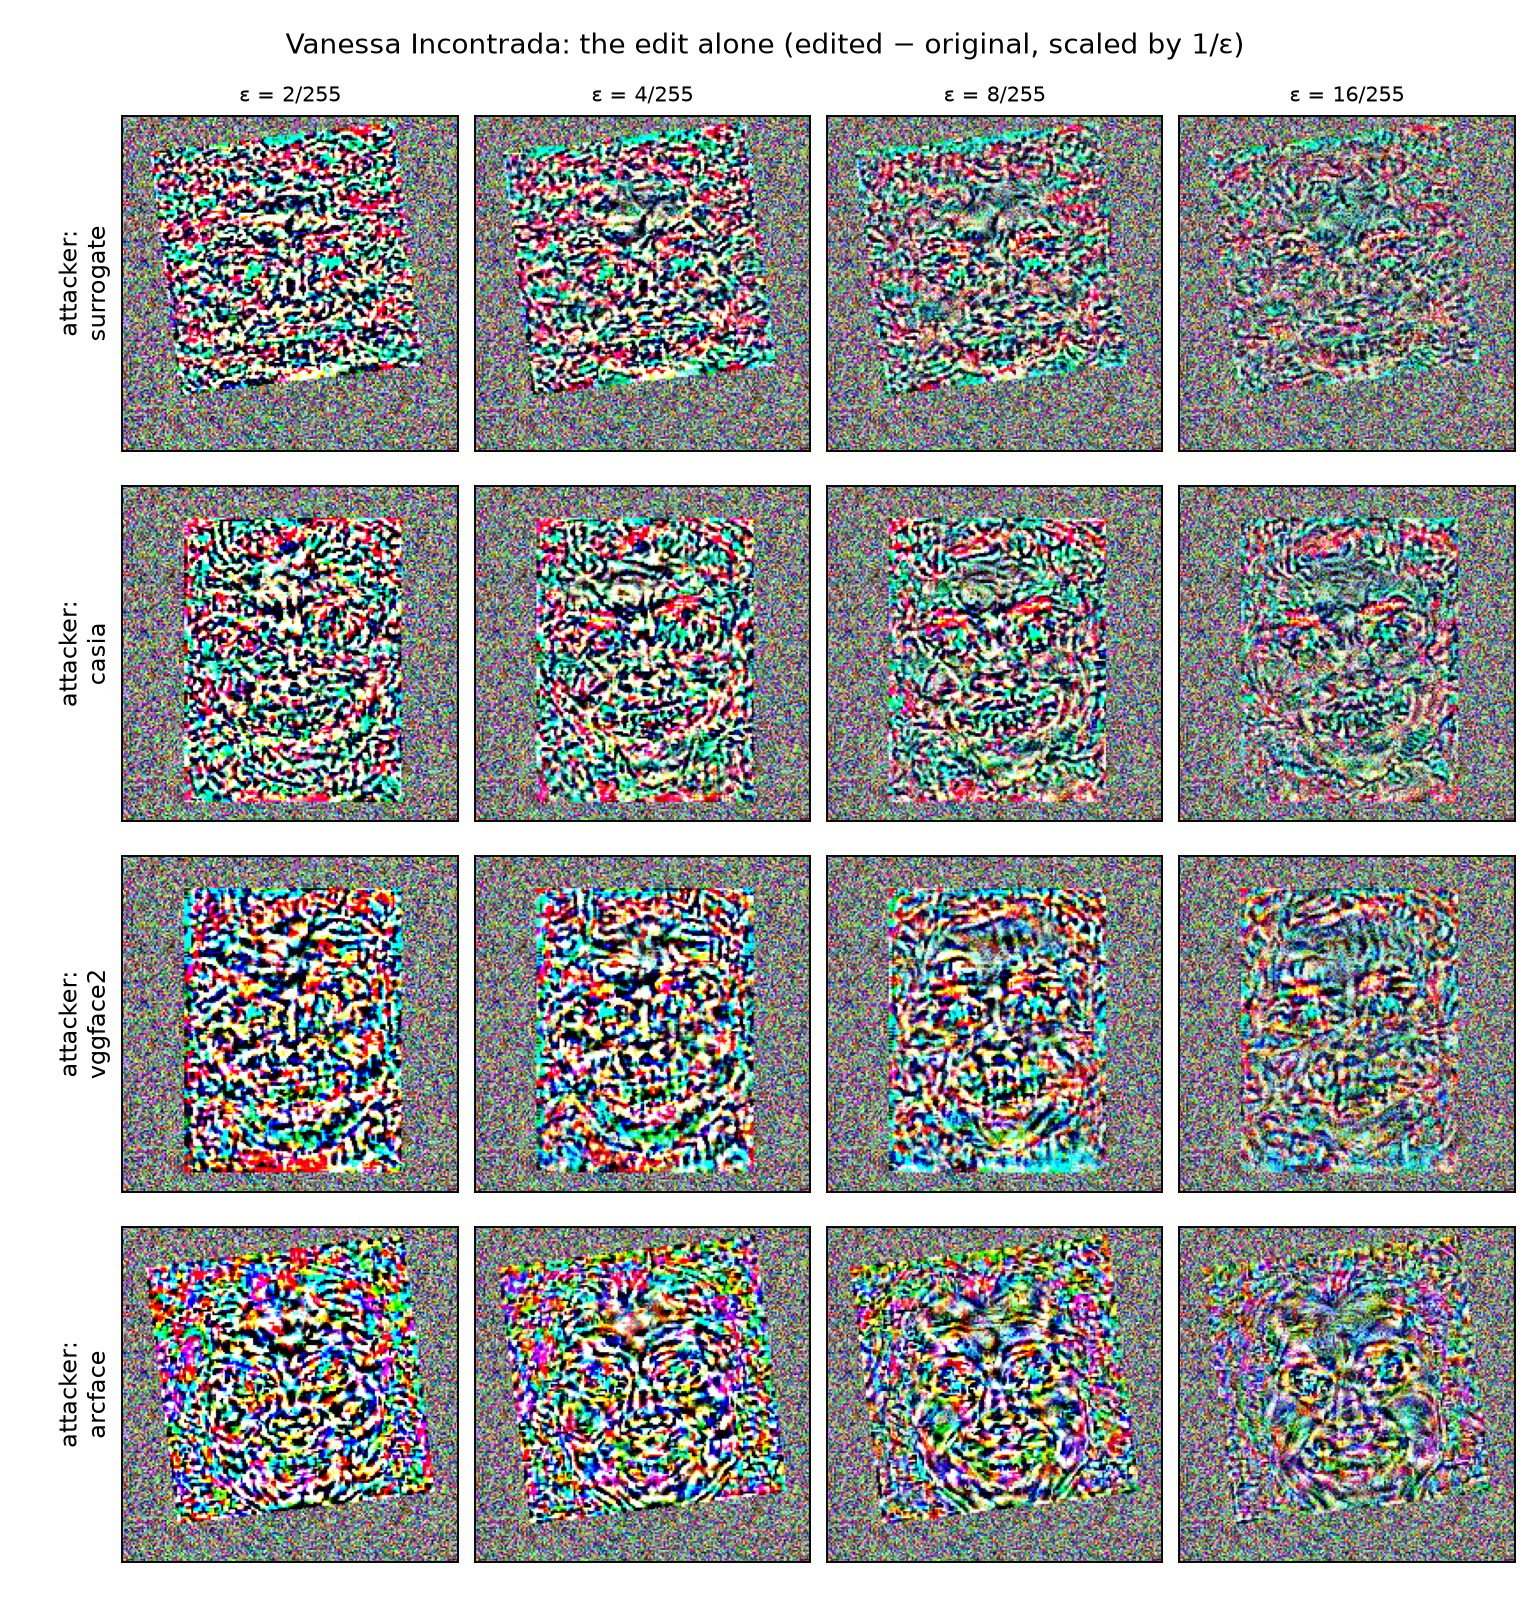
\includegraphics[width=0.38\textwidth]{figures/perturbation_0.jpg}
\caption{The edit alone (edited minus original) for the pair in Fig.~\ref{fig:example}, each column scaled by
$1/\varepsilon$.}
\label{fig:pert}
\end{figure*}

\end{document}
